\section{Ejemplo 7}

    \lipsum[1]
    
    \begin{figure}[h]
    	\centering
    	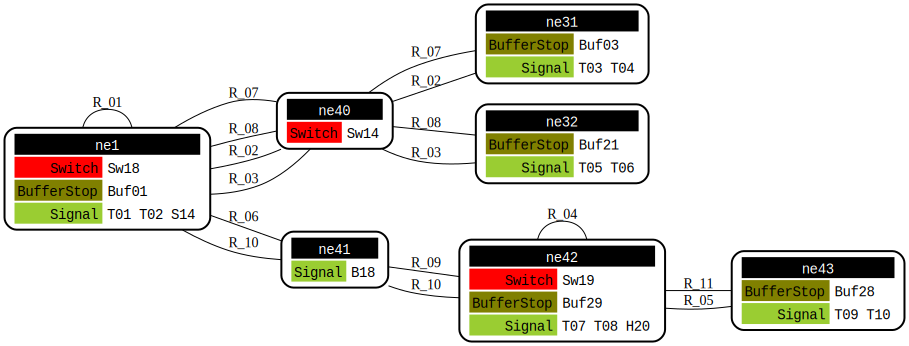
\includegraphics[width=1\textwidth]{Figuras/Graph_7}
    	\centering\caption{XXXX}
    	%\label{fig:LC_P2}
    \end{figure}
    
    \lipsum[1]

    \begin{figure}[h]
        \centering
        \includegraphics[width=1\textwidth]{resultados-obtenidos/ejemplo7/images/7_original.png}
        \centering\caption{Señalamiento original del ejemplo 7.}
        %\label{fig:LC_P2}
    \end{figure}

    \begin{figure}[h]
        \centering
        \includegraphics[width=1\textwidth]{resultados-obtenidos/ejemplo7/images/7_empty.png}
        \centering\caption{Topología ferroviaria del ejemplo 7 sin señalamiento.}
        %\label{fig:LC_P2}
    \end{figure}

    \begin{figure}[h]
        \centering
        \includegraphics[width=1\textwidth]{resultados-obtenidos/ejemplo7/images/7_step1.png}
        \centering\caption{Señalamiento generado por el RNA para proteger el fín de vía.}
        %\label{fig:LC_P2}
    \end{figure}

    \begin{figure}[h]
        \centering
        \includegraphics[width=1\textwidth]{resultados-obtenidos/ejemplo7/images/7_step2.png}
        \centering\caption{Señalamiento generado por el RNA para proteger las junturas.}
        %\label{fig:LC_P2}
    \end{figure}

    \begin{figure}[h]
        \centering
        \includegraphics[width=1\textwidth]{resultados-obtenidos/ejemplo7/images/7_step3.png}
        \centering\caption{Señalamiento generado por el RNA para proteger plataformas y cruces de vía.}
        %\label{fig:LC_P2}
    \end{figure}

    \begin{figure}[h]
        \centering
        \includegraphics[width=1\textwidth]{resultados-obtenidos/ejemplo7/images/7_step4.png}
        \centering\caption{Señalamiento generado por el RNA para proteger las máquinas de cambios.}
        %\label{fig:LC_P2}
    \end{figure}

    \begin{figure}[h]
        \centering
        \includegraphics[width=1\textwidth]{resultados-obtenidos/ejemplo7/images/7_RNA.png}
        \centering\caption{Señalamiento generado y simplificado por el RNA.}
        %\label{fig:LC_P2}
    \end{figure}
    
    \section{Señalamiento original}

    El señalamiento original, ilustrado en la Figura \ref{fig:EJ7_2}, incluye señales de parada próximas a los finales de vías absolutos (S06, S07, S08, S09, S10), señales de maniobras antes de converger en una vía principal (S02, S04, S05) y señales múltiples para cambios de vías divergentes (S01, S03).
    
    \begin{figure}[H]
    	\centering
    	\includegraphics[width=1\textwidth]{resultados-obtenidos/ejemplo7/images/7_original.png}
    	\centering\caption{Señalamiento original del ejemplo 7.}
    	\label{fig:EJ7_2}
    \end{figure}
    
    Estas señales permiten definir hasta un máximo de 8 rutas, todas ellas detalladas en la Tabla \ref{Tab:tabla_original_7}. En una primera inspección, se puede comprobar que todos los elementos ferroviarios son alcanzados por al menos una de las rutas, en al menos una dirección. Además, todos los cambios de vías son utilizados, de forma simple o compuesta. 
    
    \begin{table}[H]
        {
        \caption{Tabla de enclavamiento original del ejemplo 7.}
        \label{Tab:tabla_original_7}
        %\centering
        \begin{center}      
        	\resizebox{0.8\textwidth}{!}{
            \begin{tabular}{ c c c c c c c }
                \hline	
                    Ruta & Inicio & Final & Cambio & Plataforma & Cruce & netElement \\	
                \hline
                    R$_{01}$  & S$_{01}$ & S$_{02}$ & Sw$_{18}^{N}$ & - & - & ne$_{01}$-ne$_{41}$\\
                    R$_{02}$  & S$_{01}$ & S$_{06}$ & Sw$_{14}^{N}$+Sw$_{18}^{R}$ & - & - & ne$_{01}$-ne$_{32}$\\
                    R$_{03}$  & S$_{01}$ & S$_{07}$ & Sw$_{14}^{R}$+Sw$_{18}^{R}$ & - & - & ne$_{01}$-ne$_{31}$\\
                    R$_{04}$  & S$_{03}$ & S$_{09}$ & Sw$_{19}^{N}$ & - & - & ne$_{42}$-ne$_{43}$\\
                    R$_{05}$  & S$_{03}$ & S$_{10}$ & Sw$_{18}^{N}$+Sw$_{19}^{R}$ & - & - & ne$_{42}$-ne$_{01}$\\
                    R$_{06}$  & S$_{02}$ & S$_{08}$ & Sw$_{19}^{R}$ & - & - & ne$_{41}$-ne$_{42}$\\
                    R$_{07}$  & S$_{04}$ & S$_{10}$ & Sw$_{14}^{R}$+Sw$_{18}^{R}$ & - & - & ne$_{31}$-ne$_{01}$\\
                    R$_{08}$  & S$_{05}$ & S$_{10}$ & Sw$_{14}^{N}$+Sw$_{18}^{R}$ & - & - & ne$_{32}$-ne$_{01}$\\
                \hline
            \end{tabular}
        }
        \end{center}
     }
    \end{table}
    
    Todas las rutas abarcan mas de un \textit{netElement}, como por ejemplo la ruta R08 que comienza en la señal S05 y finaliza en la señal S10, atravesando los \textit{netElements} ne32 y ne01, utilizando los cambios de vías Sw14 y Sw18, en posición normal y reversa respectivamente.
    \subsection{Señalamiento generado por el RNA}

    \lipsum[1]
    
    \begin{table}[H]
        {
        \caption{Tabla de enclavamiento del ejemplo 7 generada por el RNA.}
        \label{Tab:tabla_generated_7}
        \centering
        \resizebox{1\textwidth}{!}{
            \begin{tabular}{ c c c c c c c }
                \hline	
                    Ruta & Inicio & Final & Cambio & Plataforma & Cruce & netElement \\	
                \hline
                    R$_{01}$  & T$_{02}$ & S$_{14}$ & - & - & - & ne$_{01}$\\
                    R$_{02}$  & T$_{04}$ & T$_{01}$ & Sw$_{14}^{R}$+Sw$_{18}^{R}$ & - & - & ne$_{31}$-ne$_{01}$\\
                    R$_{03}$  & T$_{06}$ & T$_{01}$ & Sw$_{14}^{N}$+Sw$_{18}^{R}$ & - & - & ne$_{32}$-ne$_{01}$\\
                    R$_{04}$  & T$_{08}$ & H$_{20}$ & - & - & - & ne$_{42}$\\
                    R$_{05}$  & T$_{10}$ & T$_{07}$ & Sw$_{19}^{N}$ & - & - & ne$_{43}$-ne$_{42}$\\
                    R$_{06}$  & S$_{14}$ & B$_{18}$ & Sw$_{18}^{N}$ & - & - & ne$_{01}$-ne$_{41}$\\
                    R$_{07}$  & S$_{14}$ & T$_{05}$ & Sw$_{18}^{R}$+Sw$_{14}^{N}$ & - & - & ne$_{01}$-ne$_{32}$\\
                    R$_{08}$  & S$_{14}$ & T$_{03}$ & Sw$_{18}^{R}$+Sw$_{14}^{R}$ & - & - & ne$_{01}$-ne$_{31}$\\
                    R$_{09}$  & B$_{18}$ & T$_{07}$ & Sw$_{19}^{R}$ & - & - & ne$_{41}$-ne$_{42}$\\
                    R$_{10}$  & H$_{20}$ & T$_{09}$ & Sw$_{19}^{N}$ & - & - & ne$_{42}$-ne$_{43}$\\
                    R$_{11}$  & H$_{20}$ & T$_{01}$ & Sw$_{19}^{R}$+Sw$_{18}^{N}$ & - & - & ne$_{42}$-ne$_{01}$\\
                \hline
            \end{tabular}
        }
     }
    \end{table}
    
    \lipsum[1]
    \subsection{Sistema generado por el ACG}

	En base a la red de grafos, ilustrada en la Figura \ref{fig:EJ7_8}, el ACG determinó la siguiente cantidad de elementos, tal puede visualizarse en el Código \ref{lst:EJ7_8}.
	
	\begin{lstlisting}[language = {}, caption = Cantidad de elementos a implementar por el ACG, label = {lst:EJ7_8}]
	n_netElements:7
	n_switch:3
	n_doubleSwitch:0
	n_borders:0
	n_buffers:5
	n_levelCrossings:0
	n_platforms:0
	n_scissorCrossings:0
	n_signals:13
	N : 47
	M : 40
	\end{lstlisting}
	
	El código VHDL generado por el ACG es importado en un proyecto de Vivado, donde es sintetizado e implementado para generar el bitstream que será utilizado para programar la FPGA. La cantidad de elementos de la FPGA utilizados por el sistema post-síntesis y post-implementación, así como el porcentaje de uso de la plataforma, son detallados en la Tabla \ref{Tab:tabla_ACG_7}.
	
	\begin{table}[H]
		{
			\caption{Síntesis e implementación del ejemplo 7 generado por el ACG.}
			\label{Tab:tabla_ACG_7}
			\centering
			%\small
			%\centering
			\begin{center}
				\resizebox{0.7\textwidth}{!}{
					\begin{tabular}{ c c c c }
						\hline	
						Recursos & Síntesis & Implementación & Uso \\	
						\hline
						LUT & 2102 & 2102 & 3.95\%\\
						FF & 2983 & 2983 & 2.80\%\\
						IO & 16 & 16 & 12.80\%\\
						BUFG & 1 & 1 & 3.13\%\\
						\hline
					\end{tabular}
				}
			\end{center}
		}    
	\end{table}
	
	En este ejemplo, la cantidad de recursos utilizados es baja y el tiempo de sintetización e implementación es de 35 segundos y 36 segundos respectivamente.
    \subsection{Validacion del sistema}

    Las 8 rutas del señalamiento original (Tabla \ref{Tab:tabla_original_7}) tienen 8 rutas equivalentes en el señalamiento generado por el RNA (Tabla \ref{Tab:tabla_generated_7}), tal como se puede visualizar en la Tabla \ref{Tab:tabla_validation_7}, generada automáticamente por el RNA.

    \begin{table}[H]
        {
        \caption{Equivalencias entre las rutas originales y las generadas por el RNA.}
        \label{Tab:tabla_validation_7}
        \centering
        %\small
            %\centering
            \begin{center}
            \resizebox{0.7\textwidth}{!}{
            \begin{tabular}{ c c c c }
                \hline	
                    Original & Señales & RNA & Señales \\	
                \hline
                    R$_{01}$ & S$_{01}$-S$_{02}$ & R$_{06}$ & S$_{14}$-B$_{18}$ \\
                    R$_{02}$ & S$_{01}$-S$_{06}$ & R$_{07}$ & S$_{14}$-T$_{05}$ \\
                    R$_{03}$ & S$_{01}$-S$_{07}$ & R$_{08}$ & S$_{14}$-T$_{03}$ \\
                    R$_{04}$ & S$_{03}$-S$_{09}$ & R$_{09}$ & B$_{18}$-T$_{07}$ \\
                    R$_{05}$ & S$_{03}$-S$_{10}$ & R$_{11}$ & H$_{20}$-T$_{09}$ \\
                    R$_{06}$ & S$_{02}$-S$_{08}$ & R$_{10}$ & H$_{20}$-T$_{01}$ \\
                    R$_{07}$ & S$_{04}$-S$_{10}$ & R$_{02}$ & T$_{04}$-T$_{01}$ \\
                    R$_{08}$ & S$_{05}$-S$_{10}$ & R$_{03}$ & T$_{06}$-T$_{01}$ \\
                \hline
            \end{tabular}
            }
            \end{center}
        }    
    \end{table}
    
     Las rutas R1, R4 y R5 (Tabla \ref{Tab:tabla_generated_7}) generadas por el RNA que no tienen equivalencias en el señalamiento original (Tabla \ref{Tab:tabla_original_7}) se deben a que el RNA creó señales extras. Las señales T02, T08 y T10 fueron creadas por el RNA para proteger los finales de vía absolutos. La Ruta R1 fue establecida por el RNA al crear la señal T02 para proteger el final de vía del \textit{netElement} ne01, creando una ruta con la señal S14. La Ruta R4 fue establecida por el RNA al crear la señal T08 para proteger el final de vía del \textit{netElement} ne42, creando una ruta con la señal S14. La ruta R4 añade una parada intermedia entre las rutas R4 y R5 del señalamiento original, previo al cambio de vías Sw19. La Ruta R5 fue establecida por el RNA al crear la señal T10 para proteger el final de vía del \textit{netElement} ne43, creando una ruta con la señal T07. Estos elementos ferroviarios no se encontraban protegidos en el señalamiento original, además que particionar las rutas R4 y R5 originales en R4+R10 y R4+R11 respectivamente incrementa la mobilidad de la red.